\documentclass[11pt,a4paper]{report}
\usepackage[utf8]{inputenc}
\usepackage[french]{babel}
\usepackage[T1]{fontenc}
\usepackage{amsmath}
\usepackage{amsfonts}
\usepackage{amssymb}
\usepackage{makeidx}
\usepackage{svg}
\author{Frantzen Christian Marius Küpper}
\title{INFO-H-303 : Base de données\\
		Projet : Annuaire d'établissements horeca}
\begin{document}
\maketitle
\section*{Modèle entité-association}

\begin{figure}[h]
  \centering
  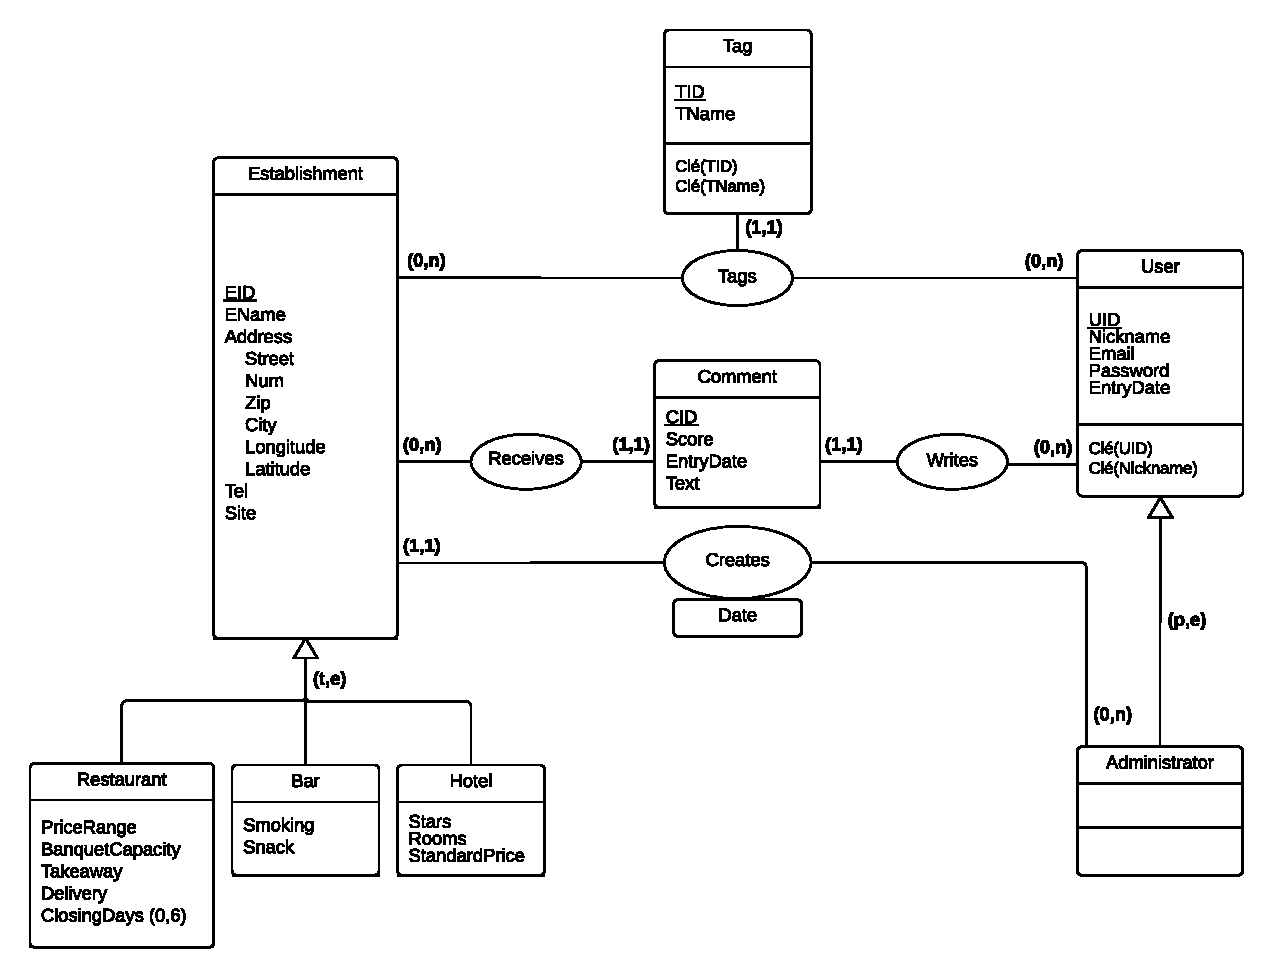
\includegraphics[width=\textwidth]{modelEA.pdf}
  \caption{Modèle entité-association}
\end{figure}


\subsection*{Contraintes d'intégrité}

\begin{itemize}
\item Un \textit{User} peut commenter plusieurs fois le même \textit{Establishment} à des dates différentes. 
\item Un \textit{User} ne peut pas apposer le même \textit{Tag} plusieurs fois sur le même \textit{Establishment}.
\item Deux \textit{User} ne peuvent pas avoir le même \textit{Nickname} (Les \textit{Adminisitrator} sont aussi des User).
\item L'\textit{EntryDate} d'un \textit{Adminisitrator} doit être strictement supérieure à l'\textit{EntryDate} de l'\textit{Establishment} qu'il a créé.
\item L'\textit{EntryDate} d'un \textit{Comment} doit être strictement supérieure à l'\textit{EntryDate} du User qui le fait ainsi que l'\textit{EntryDate} de l'\textit{Establishment} sur lequel il est fait. 
\item Le \textit{Score} d'un \textit{Comment} est un entier compris entre 0 et 5.
\item Les \textit{Stars} d'un \textit{Hotel} est un entier compris entre 0 et 5.
\item Le nombre \textit{Rooms} d'un \textit{Hotel} doit être strictement positif. 
\item Le \textit{StandardPrice} d'un \textit{Hotel} doit être strictement positif. 
\item Le \textit{PriceRange} d'un \textit{Restaurant} doit être strictement positif. 
\item Le \textit{BanquetCapacity} d'un \textit{Restaurant} doit être positif. 
\item Deux \textit{Tag} ne peuvent pas avoir le même \textit{TName}.
\end{itemize}
\subsection*{Remarques}
Si un \textit{Restaurant} ne veut pas organiser de banquet, il spécifie sa \textit{BanquetCapacity} comme étant 0.

\section*{Modèle relationnel}
\noindent

Establishment(\underline{EID}, EName, Street, Num, Zip, City, Longitude, Latitude, Tel, Site, \underline{UID}, EntryDate)
\begin{itemize}
\item UID référence User.UID (représente le createur de l'établissement)\\
\end{itemize}

Restaurant(\underline{EID}, PriceRange, BanquetCapacity, Takeaway, Delivery)
\begin{itemize}
\item EID référence Establishment.EID\\
\end{itemize} 

RestaurantClosingDays(\underline{EID}, ClosingDay, Hour)
\begin{itemize}
\item EID référence Establishment.EID\\
\end{itemize}

Bar(\underline{EID}, Smoking, Snack)
\begin{itemize}
\item EID référence Establishment.EID\\
\end{itemize}

Hotel(\underline{EID}, Stars, Rooms, StandardPrice)
\begin{itemize}
\item EID référence Establishment.EID\\
\end{itemize}

User(\underline{UID}, \underline{Nickname}, Email, Password, EntryDate, Admin)\\ 

Comment(\underline{CID}, \underline{UID}, \underline{EID}, Score, EntryDate, Text)
\begin{itemize}
\item UID référence User.UID
\item EID référence Establishment.EID
\item (UID,EID,EntryDate) est unique et donc également une clé de cette relation\\
\end{itemize}

Tag(\underline{TID}, \underline{TName})\\ \\

EstablishmentTag(\underline{TID, EID, UID})
\begin{itemize}
\item TID référence Tag.TID
\item EID référence Establishment.EID
\item UID référence User.UID\\
\end{itemize}

\section*{Remarques}
\noindent

User.Admin est soit True, soit False (Seul les User avec User.Admin = True a les droits de créer, supprimer et modifier des Establishment)

Pour le commentaire sur un établissement Comment.EntryDate > Establishment.EntryDate et Comment.EntryDate > User.EntryDate

0 <= Comment.Score <= 5

Pour tout Establishment il existe soit un Restaurant, soit un Bar, soit un Hotel

Pour chaque Restaurant il existe un RestaurantClosingDays

0 <= Hotel.Stars <= 5

Hotel.Rooms >= 0

Hotel.StandartPrice > 0

Restaurant.BanquetCapacity >= 0

Restaurant.PriceRange > 0

RestaurantClosingDays.Hour est soit "AM", soit "PM" (matin / après-midi)




\section*{Hypothèses}
\noindent

\begin{itemize}
\item \underline{Deux User ne peuvent pas avoir le même Nickname:} L'interface doit permettre de consulter la fiche de chaque utilisateur, un utilisateur qui cherche le profil de son ami ne peut pas différencer entre deux utilisateur avec le même Nickname puisque le Nickname est la seule donnée visible (pas d'image de profil, etc ...).\\
\end{itemize}



\begin{itemize}
\item \underline{Un admin ne peut pas modifier des commentaires et labels:} TODO:justifier
\end{itemize}

\end{document}